\chapter{RESULTS AND ANALYSIS}
\label{ch:results}

% State main findings in words FIRST, then go into details. Use subheadings.
% Every claim here must be backed by a row in benchmark_results or a figure
% generated from it. No prose claims without a number behind them.
% Target length: ~1,500-2,500 words.

In the noiseless simulator benchmark, retrieval accuracy mainly depended on the
embedding dimension, not on whether the engine was classical or quantum. The
three classical baselines returned identical rankings and tied at MRR 0.829, and
every engine improved as the dimension rose from 64 to 256. The swap test
reproduced the classical ranking at dimension 256 (MRR 0.975) and recovered at
lower dimensions as shots increased. Grover with a hardcoded oracle matched the
theoretical $\lfloor(\pi/4)\sqrt{N}\rfloor$ oracle count, but its probabilistic
measurement stopped at MRR 0.955 at dimension 256. Grover with quantum state
preparation was weakest (MRR 0.559). The hybrid engine effectively tied the
classical baseline (MRR 0.823) by using HNSW for search and the swap test only
for reranking.

These accuracy results should not be read as predictions for a large, noisy
quantum computer. The simulator removes gate noise, measurement error beyond
finite-shot sampling, queueing, and hardware latency. The measured pattern still
answers the algorithmic question under controlled conditions, but real hardware
would be expected to degrade the quantum-engine accuracy unless error rates and
circuit depth are low enough for the chosen workload.

\section{Accuracy Across Engines}
\label{sec:results:mrr}

% MRR per engine, broken out by dimension and shots where relevant. Use the
% same table layout as the frontend BenchmarkResults component.

\begin{table}[ht]
  \centering
  \caption[Mean Reciprocal Rank by engine and dimension]{Average Mean
  Reciprocal Rank (MRR) by engine and embedding
  dimension, over the twenty benchmark queries. Higher is better: an MRR of
  1.000 means the correct image was ranked first for every query. Quantum
  cells average over the three shot counts (512, 1024, 2048); the shot
  dependence is examined separately below. The IBM hardware run is reported
  in Section~\ref{sec:results:ibm}.}
  \label{tab:mrr}
  \begin{tabularx}{\linewidth}{Xcccc}
    \toprule
    & \multicolumn{3}{c}{\textbf{MRR by dimension}} & \\
    \cmidrule(lr){2-4}
    \textbf{Engine} & \textbf{64} & \textbf{128} & \textbf{256} & \textbf{Avg} \\
    \midrule
    Brute-force cosine          & 0.655 & 0.858 & 0.975 & 0.829 \\
    FAISS flat                  & 0.655 & 0.858 & 0.975 & 0.829 \\
    FAISS HNSW                  & 0.655 & 0.858 & 0.975 & 0.829 \\
    \addlinespace
    Swap test                   & 0.470 & 0.738 & 0.975 & 0.728 \\
    Grover (hardcoded oracle)   & 0.546 & 0.776 & 0.955 & 0.759 \\
    Grover (quantum state prep) & 0.404 & 0.551 & 0.722 & 0.559 \\
    \addlinespace
    Hybrid (HNSW + swap test)   & 0.635 & 0.858 & 0.975 & 0.823 \\
    \bottomrule
  \end{tabularx}
\end{table}

Table~\ref{tab:mrr} shows that brute-force cosine, FAISS flat, and FAISS HNSW
all scored MRR 0.829 and produced the same query-by-query ordering. This is
expected: brute force and FAISS flat are exact searches over the same twenty
unit vectors, and HNSW's approximation does not matter on a graph this small. We
treat the brute-force result as the reference ordering.

Embedding dimension had the strongest effect on accuracy. Every engine improved
from dimension 64 to 256, and the classical baseline moved through 0.655, 0.858,
and 0.975. Truncating CLIP vectors discards information that separates
near-neighbours; restoring dimensions recovers it. The lower dimensions are
therefore a simulation trade-off, not the configuration a retrieval system would
prefer.

The swap test illustrates how a quantum estimator approaches the exact answer as
its measurement budget grows. At dimension 256 it matched the best classical
score exactly (MRR 0.975 at every shot count), because the overlaps it estimates
are well separated and even a coarse estimate ranks them correctly. At dimension
128, where neighbours are closer together, accuracy depended on how finely we
measured: MRR rose from 0.642 at 512 shots to 0.688 at 1024 and 0.883 at 2048.
The swap test estimates the squared overlap $|\langle\psi|\phi\rangle|^2$ from
a finite number of measurements, so additional shots reduce the sampling noise
and sharpen the ranking. This shot-versus-accuracy trade-off, rather than a
fixed limit of the method itself, explains the swap test's lower average of
0.728: the average is pulled down by the low-dimension, low-shot configurations
that a practical deployment would not choose.

The two Grover engines separate sharply. The hardcoded-oracle version reached
MRR 0.955 at dimension 256, just short of the best classical score of 0.975,
because the marked state is still measured probabilistically. The quantum
state-preparation variant was weakest at every dimension and averaged 0.559:
state preparation and
per-candidate swap tests add noise before Grover amplifies the chosen index. The
hybrid takes the opposite approach. HNSW chooses the candidates, and the swap
test reranks only that shortlist, so it stayed close to the baseline (MRR 0.823,
and 0.975 at dimension 256).

\section{Quantum Resource Cost}
\label{sec:results:cost}

% Circuit depth, qubit count, oracle calls. This section answers RQ2 (Grover
% scaling) and supports the practicality framing on RQ3.

Because the quantum engines run on a classical simulator, their wall-clock time
measures simulation overhead rather than the cost of a real quantum device
(Section~\ref{sec:results:walltime} returns to this). The hardware-neutral way
to compare the engines is therefore to count the operations each one performs per
query and the resources its circuit would demand on a real device.
Table~\ref{tab:opcount} reports the first of these: the number of similarity
comparisons or oracle calls each engine makes for a single query over the
twenty-image dataset.

\begin{table}[ht]
  \centering
  \caption[Operations per query and complexity class]{Operations per query and
  algorithmic complexity for each engine over
  the twenty-image dataset ($N=20$). The operation count is the cross-engine
  scaling metric; it is independent of hardware. Here $M$ denotes the number of
  candidates the hybrid engine reranks.}
  \label{tab:opcount}
  \begin{tabularx}{\linewidth}{Xcc}
    \toprule
    \textbf{Engine} & \textbf{Operations / query} & \textbf{Complexity} \\
    \midrule
    Brute-force cosine          & 20 & $O(N)$ \\
    FAISS flat                  & 20 & $O(N)$ \\
    FAISS HNSW                  & 5  & $O(\log N)$ approx. \\
    \addlinespace
    Swap test                   & 20 & $O(N)$ \\
    Grover (hardcoded oracle)   & 4  & $O(\sqrt{N})$ \\
    Grover (quantum state prep) & 4  & $O(\sqrt{N})$ \\
    \addlinespace
    Hybrid (HNSW + swap test)   & 10 & $O(\log N + M)$ \\
    \bottomrule
  \end{tabularx}
\end{table}

Grover was the only engine whose per-query cost was sublinear in the dataset
size. The exact classical engines and the standalone swap test each performed one
comparison per stored vector, twenty in total, while FAISS HNSW reached its
answer in about five graph hops and the hybrid engine made ten comparisons (one
HNSW shortlist followed by a swap-test rerank of the survivors). Both Grover
engines used four oracle calls, and this count is exactly what the theory
predicts once the index padding is accounted for. Grover addresses an index
register whose length is a power of two, so the twenty images are padded to the
next power of two, $N' = 32$, which is why the Grover circuits used five qubits
($\lceil \log_2 32 \rceil = 5$). The optimal number of Grover iterations for an
unstructured search of $N'$ items is $\lfloor (\pi/4)\sqrt{N'} \rfloor$, and for
$N' = 32$ this evaluates to $\lfloor 4.44 \rfloor = 4$, matching the measured
count. Figure~\ref{fig:oracle_scaling} places this verified point on the
theoretical curve.

\begin{figure}[ht]
  \centering
  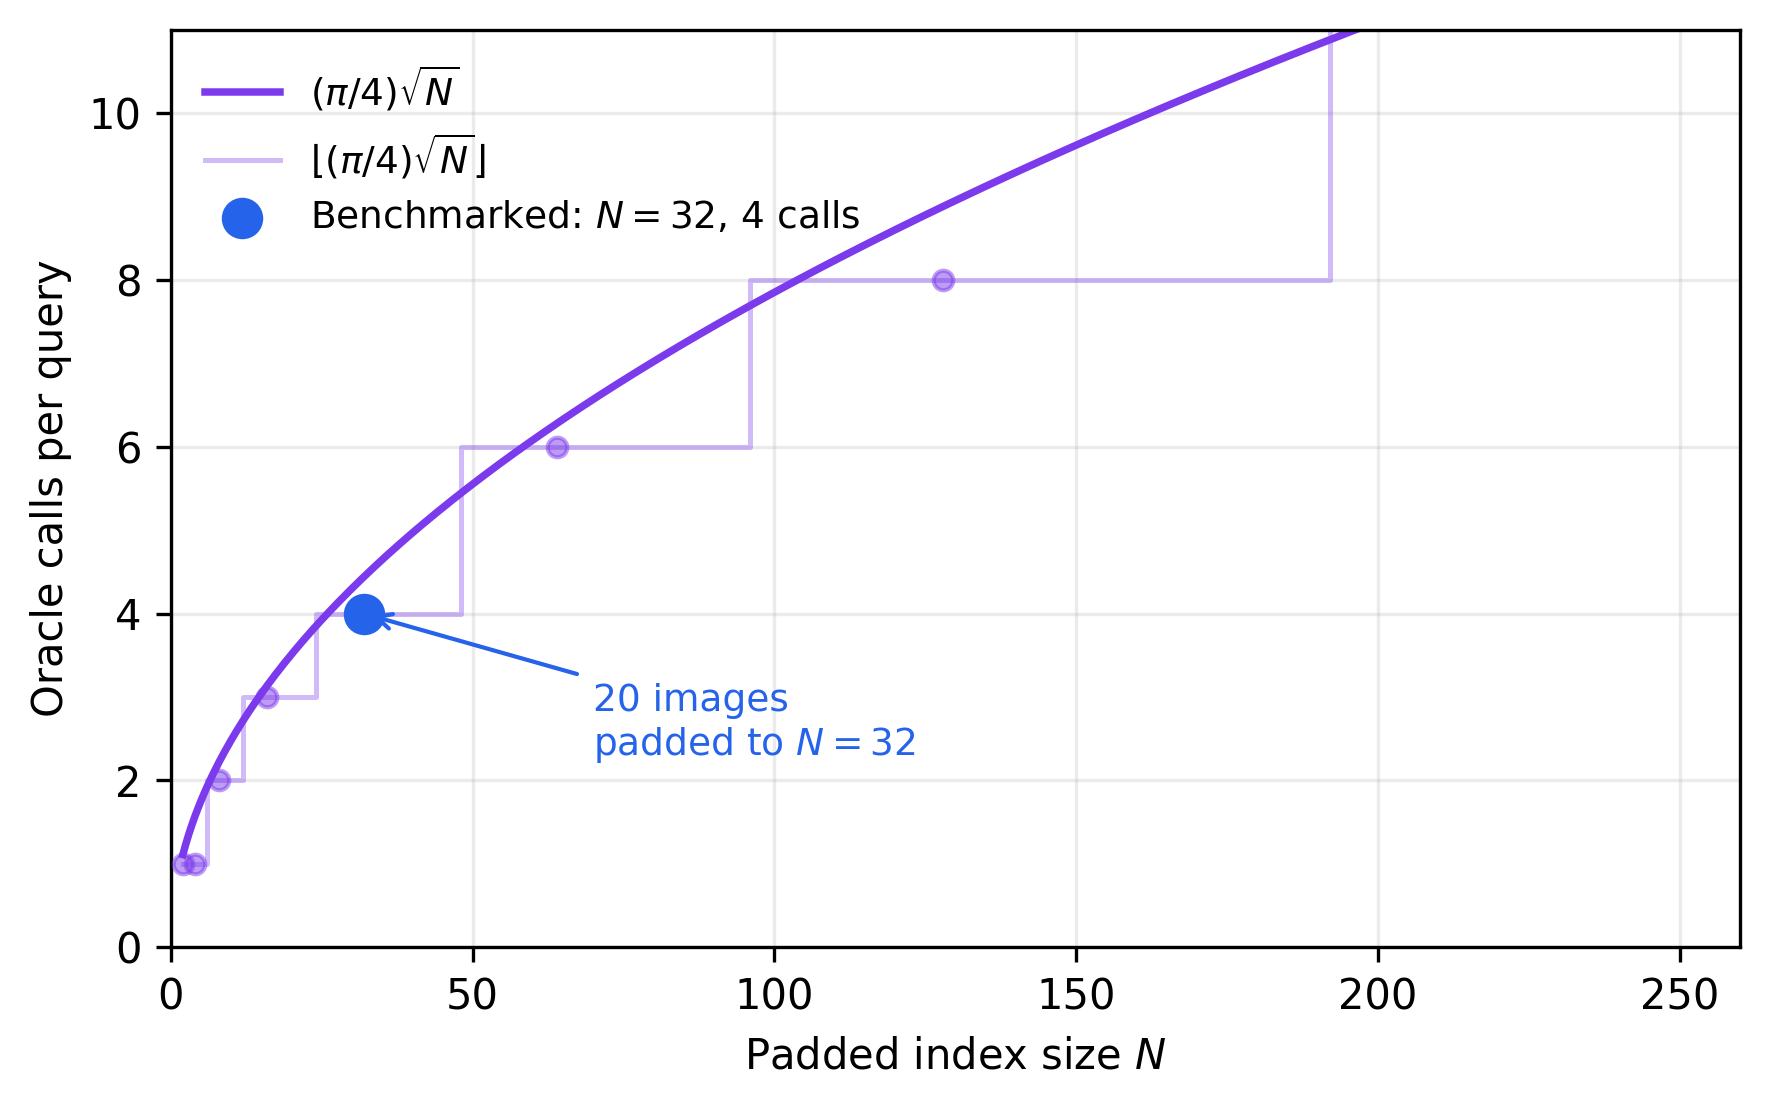
\includegraphics[width=0.8\linewidth]{figures/oracle_scaling.png}
  \caption[Grover oracle-call scaling]{Theoretical Grover oracle-call count
  $\lfloor (\pi/4)\sqrt{N} \rfloor$ as a function of the padded index size $N$,
  with a marker at the single size we benchmarked ($N = 32$, four oracle calls).
  We ran one dataset size, so this confirms the count at a single point on the
  curve rather than tracing the curve empirically.}
  \label{fig:oracle_scaling}
\end{figure}

The two quantum families differ sharply in what they encode, and
Table~\ref{tab:circuitcost} shows the consequence for circuit width and depth.
Grover encodes the candidate \emph{index}, so its width stayed fixed at five
qubits regardless of the embedding dimension; its cost instead appears as depth,
around fifty gate layers, because each of the four iterations applies an oracle
and a diffusion operator in sequence. The swap test and the hybrid engine encode
the candidate \emph{vectors}, so their width grew with the embedding dimension as
$1 + 2\lceil \log_2 d \rceil$ qubits, from thirteen at dimension 64 to seventeen
at dimension 256, while their circuits stayed shallow (depth nine to eleven). On
near-term hardware both costs matter: more qubits are harder to allocate, and
greater depth gives decoherence more time to corrupt the state, which is the
practical reason the deep Grover circuits would be the harder of the two to run
faithfully on a real device.

\begin{table}[ht]
  \centering
  \caption[Quantum circuit width and depth]{Circuit width and depth for the
  quantum engines, from the compiled
  circuits. The swap test and the hybrid engine share the same circuit metrics
  because the hybrid reuses the swap-test circuit. Grover's width is set by the
  padded index register, not the embedding dimension, so it is constant.}
  \label{tab:circuitcost}
  \begin{tabularx}{\linewidth}{Xccc}
    \toprule
    \textbf{Engine (dimension)} & \textbf{Qubits} & \textbf{Circuit depth} \\
    \midrule
    Swap test / Hybrid, dim 64   & 13 & 9 \\
    Swap test / Hybrid, dim 128  & 15 & 10 \\
    Swap test / Hybrid, dim 256  & 17 & 11 \\
    \addlinespace
    Grover (both variants), any dim & 5 & $\approx 50$ \\
    \bottomrule
  \end{tabularx}
\end{table}

These counts also expose the assumption hidden inside Grover's sublinear figure.
The four oracle calls measure only the search once the data is already encoded in
the oracle; they do not include the cost of building that oracle. Our hardcoded
oracle computes the nearest neighbour classically and then marks it, so the
twenty comparisons Grover appears to save have in effect been paid before the
circuit runs. This is the qRAM caveat set out in Section~\ref{sec:method:engines}:
a genuine quantum speed-up for search would require loading the dataset into a
quantum-accessible memory, which is itself an unsolved cost. The swap test and
hybrid engines make the opposite trade, paying their cost openly in qubits and in
one circuit execution per candidate. Section~\ref{sec:results:discussion} returns
to what this means for the practicality question.

\section{Wall-Clock Behaviour (Within-Engine Only)}
\label{sec:results:walltime}

% IMPORTANT: per docs/NOTES.md, wall-clock is NOT a valid cross-engine metric on
% a simulator. State this in the first sentence to avoid the reader misreading
% the numbers.

Wall-clock time cannot be compared across engines in this study, and
Table~\ref{tab:walltime} should be read only one row at a time. The reason is
that the quantum engines did not run on a quantum computer: they ran on a
classical statevector simulator, which represents the full quantum state in
ordinary memory and so does work that grows exponentially with the number of
qubits. The times for the quantum engines therefore measure the cost of
\emph{simulating} a circuit on a CPU, not the latency a real quantum processor
would incur, and putting them next to the classical millisecond figures would
compare two unrelated quantities. The within-engine comparison across dimension
is meaningful, because there the hardware is held fixed and only the problem size
changes.

\begin{table}[ht]
  \centering
  \caption[Mean query time by engine and dimension]{Mean total time per query,
  in milliseconds, by engine and embedding
  dimension. The three classical engines completed in well under a millisecond
  (0.2 to 0.6 ms) and are shown as ``$<1$''. The quantum and hybrid times are
  simulator times on a CPU and are \emph{not} comparable to the classical
  figures or to real quantum hardware; they are reported only to show how each
  engine's simulation cost scales with dimension.}
  \label{tab:walltime}
  \begin{tabularx}{\linewidth}{Xccc}
    \toprule
    & \multicolumn{3}{c}{\textbf{Mean time per query (ms)}} \\
    \cmidrule(lr){2-4}
    \textbf{Engine} & \textbf{dim 64} & \textbf{dim 128} & \textbf{dim 256} \\
    \midrule
    Brute-force cosine          & $<1$ & $<1$  & $<1$ \\
    FAISS flat                  & $<1$ & $<1$  & $<1$ \\
    FAISS HNSW                  & $<1$ & $<1$  & $<1$ \\
    \addlinespace
    Swap test                   & 993  & 4764  & 21555 \\
    Grover (hardcoded oracle)   & 19   & 20    & 19 \\
    Grover (quantum state prep) & 3399 & 6916  & 7453 \\
    Hybrid (HNSW + swap test)   & 254  & 1134  & 5255 \\
    \bottomrule
  \end{tabularx}
\end{table}

Read row by row, the table reflects circuit size. The swap test and hybrid
slowed sharply as dimension rose, because each doubling adds two qubits to the
amplitude encoding and quadruples the simulator state. The swap test grew from
about one second per query at dimension 64 to roughly twenty-two seconds at
dimension 256. Hardcoded Grover stayed near twenty milliseconds because it uses
the same five-qubit index register at every dimension. The simulator, not the
algorithm, set the cap of 256 dimensions.

\section{IBM Hardware Sanity Check}
\label{sec:results:ibm}

% The dimension-2, 2-candidate validation run. Frame as: "we want to confirm
% the swap test circuit behaves the same on real hardware as on the simulator,
% within shot noise". Do NOT make scaling claims from this.

All of the quantum results above were produced on a simulator. To confirm that
the swap-test pipeline also runs on a physical quantum processor, we executed the
hybrid engine once on real IBM Quantum hardware through the IBM Quantum cloud
service. This run was deliberately tiny: it used two-dimensional vectors, two
candidates per query, and thirty-two measurement shots, across the same twenty
queries, and it consumed eighty seconds of the limited free-tier quota. We treat
it as a sanity check on the execution path, not as a benchmark, and it is kept
separate from the simulator results for that reason.

The run achieved MRR 0.125, far below the simulator figures. This reflects the
configuration rather than the method: two-dimensional vectors remove most
semantic information, two candidates make the task close to a coin toss, and
thirty-two shots give a noisy overlap estimate before device noise is added. The
run establishes only that the hardware path works end to end. It does not
support accuracy or scaling claims.

\section{Discussion}
\label{sec:results:discussion}

% Tie results back to the three research questions. Answer each one explicitly:
% "RQ1: yes, swap test reproduces classical ranking at >= X shots. RQ2: yes,
% oracle count matches theory to within Y%. RQ3: no - HNSW beats Grover even
% under ideal-qRAM assumptions at N >= Z."

\textbf{RQ1 (Accuracy).} The swap test reproduced the retrieval accuracy of
classical cosine similarity once it was given enough measurement shots, and the
shot budget it needed depended on how close the candidate vectors were. At
dimension 256, where neighbours are well separated, it matched the classical MRR
of 0.975 at every shot count we tried, including the smallest. At dimension 128
it reached classical accuracy only at the highest setting, rising to 0.883 at
2048 shots from 0.642 at 512, and at dimension 64 it remained below the classical
baseline even at 2048 shots. The pattern is consistent with the swap test being a
sampled estimate of vector overlap: the harder the discrimination, the more shots
are required to resolve it. \emph{Yes: the swap test reproduces classical
retrieval accuracy given a sufficient shot budget, and the budget required grows
as the embedding dimension, and hence the separation between neighbours, falls.}

\textbf{RQ2 (Scaling).} Our Grover implementation used four oracle calls per
query, which is exactly the theoretical optimum $\lfloor (\pi/4)\sqrt{N'}
\rfloor$ for the padded index size $N' = 32$, as set out in
Section~\ref{sec:results:cost}. The match was exact rather than approximate.
The qualification is that we benchmarked only one dataset size, so we confirmed
the formula at a single point rather than tracing the scaling curve across a
range of $N$. \emph{Yes: at the size we tested, the oracle-call count matched the
theoretical $\lfloor (\pi/4)\sqrt{N} \rfloor$ optimum exactly, though a single
dataset size cannot demonstrate the full curve.}

\textbf{RQ3 (Practicality).} No engine that performed the search on a quantum
circuit beat the classical HNSW baseline on this dataset. HNSW reached the full
brute-force accuracy of 0.829 in about five graph hops, while the standalone
quantum engines were either less accurate or, in Grover's case, dependent on a
classically precomputed oracle. The one quantum-containing engine that matched
the baseline, the hybrid, did so precisely because the classical index performed
the search and the swap test only reranked a shortlist; its accuracy is inherited
from HNSW, not produced by the quantum step. \emph{We found no condition under
which a quantum search engine outperformed the HNSW baseline on this dataset; the
strongest quantum-containing engine matched it only by delegating the search
itself to the classical index.}

\textbf{RQ4 (Fit).} The resource accounting in
Section~\ref{sec:results:cost} points to a reason for the RQ3 result.
Grover's sublinear oracle count is genuine, but it measures the search after the
data has been loaded into the oracle; constructing that oracle, or an equivalent
quantum-accessible memory, reintroduces a cost linear in the dataset size. Vector
retrieval is dominated by exactly this data-loading step, because answering a
query means comparing against many stored items. Quantum advantage, by contrast,
is generally argued to concentrate on compute-bound problems that do heavy
processing over small inputs rather than on data-bound problems that must read a
large dataset~\cite{aaronson2015readfine,hoefler2023practicality}. \emph{On both
our evidence and the structure of the problem, the search part of cross-modal
vector retrieval is not a good match for quantum advantage under the methods we
tested. A quantum step is more plausible as a reranker for a small shortlist than
as the engine that scans or indexes the whole dataset.}

\section{Limitations}
\label{sec:results:limitations}

% Be honest. Small dataset (20 images), simulator-only quantum execution,
% truncated CLIP embeddings, classical-precomputed Grover oracle.

Several constraints bound the results. The dataset has twenty images and one
query per image, which kept the sweep simulable and the target unambiguous but
limited statistical power. HNSW did not have enough vectors to exercise its
approximation, so its match with exact search holds only here. Except for the
IBM sanity check, the quantum engines ran on a classical simulator, so the
results do not measure present-day hardware noise or latency. Embeddings were
truncated from 512 to at most 256 dimensions to fit the qubit budget, so absolute
MRR values are comparisons under a shared handicap. Grover used a classically
precomputed oracle, and its oracle-call scaling was checked at one dataset size,
not across a range.
